\chapter{Results}
    In this chapter we will cover different part of the results. First we will go through the leg pattern motion to see how they move and how accurate they are with previous paper \cite{mo_main_paper}. Then we will focus on the robot displacement and the simulation. 
    \section{Legs patterns}
        This is the basic block of results we need in order to build the other modules. We need to be able to encode the 15 sequences that a multistable joint can have as seen on Figure \ref{fig:sequences}. We will go through the sequences here. Each time we will have the same structure, a Figure on the left representing the Final State Machine or the order of motion from the middle and the top block, which can vary from forward and backward movement. On the right we will have a Figure which plot the position of the leg in x-axis and z-axis with respect to the position off the actuator represented by the color of the line.
        \begin{figure}[h]
            \centering
            \begin{subfigure}{.2\textwidth}
            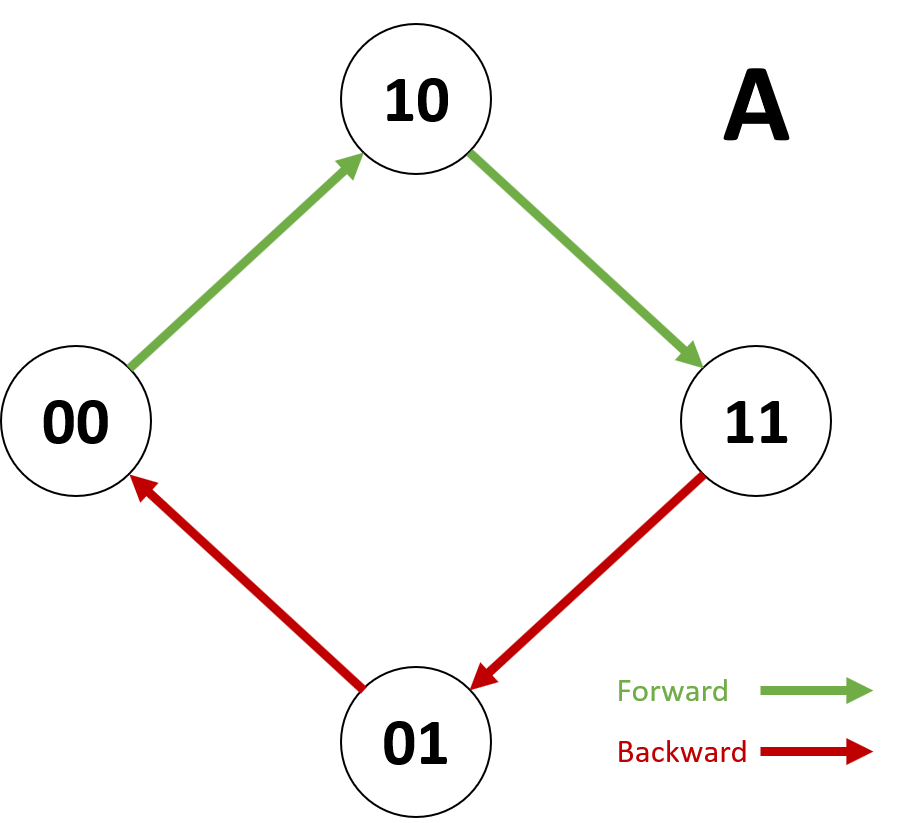
\includegraphics[width=\textwidth]{images/S_A.png}
            \end{subfigure}%
            \begin{subfigure}{.6\textwidth}
            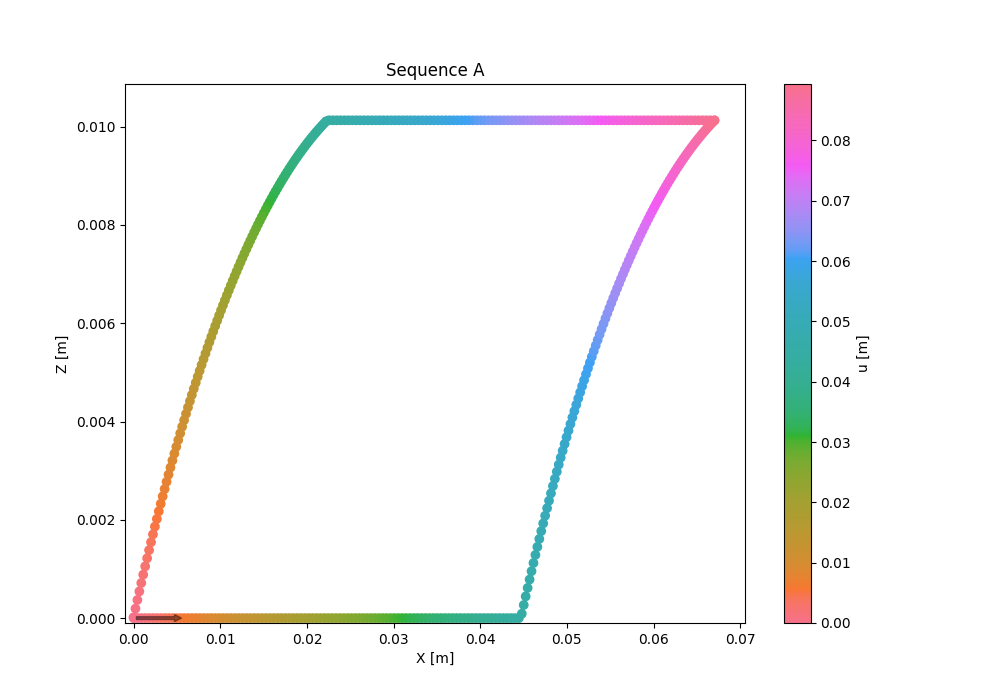
\includegraphics[width=\textwidth]{images/A.png}
            \end{subfigure}
            \caption{Sequence A is one of the simplest sequence where the middle block is moving first in forward and backward motion. This leads to a hysteresis as we can see. The arrow shows the direction of motion, which is counter-clockwise. Sequence B (Figure \ref{fig:appendix_seq_B}) is identical except that it goes clockwise.}
        \end{figure}
        
        
        \begin{figure}[h]
            \centering
            \begin{subfigure}{.2\textwidth}
            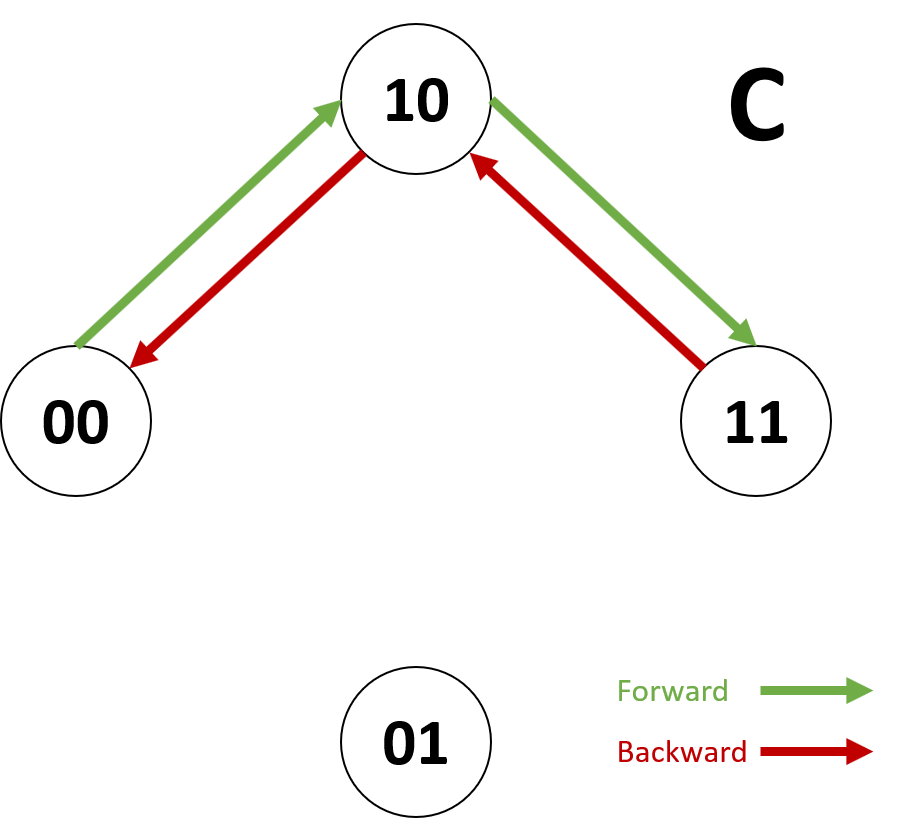
\includegraphics[width=\textwidth]{images/S_C.png}
            \end{subfigure}%
            \begin{subfigure}{.6\textwidth}
            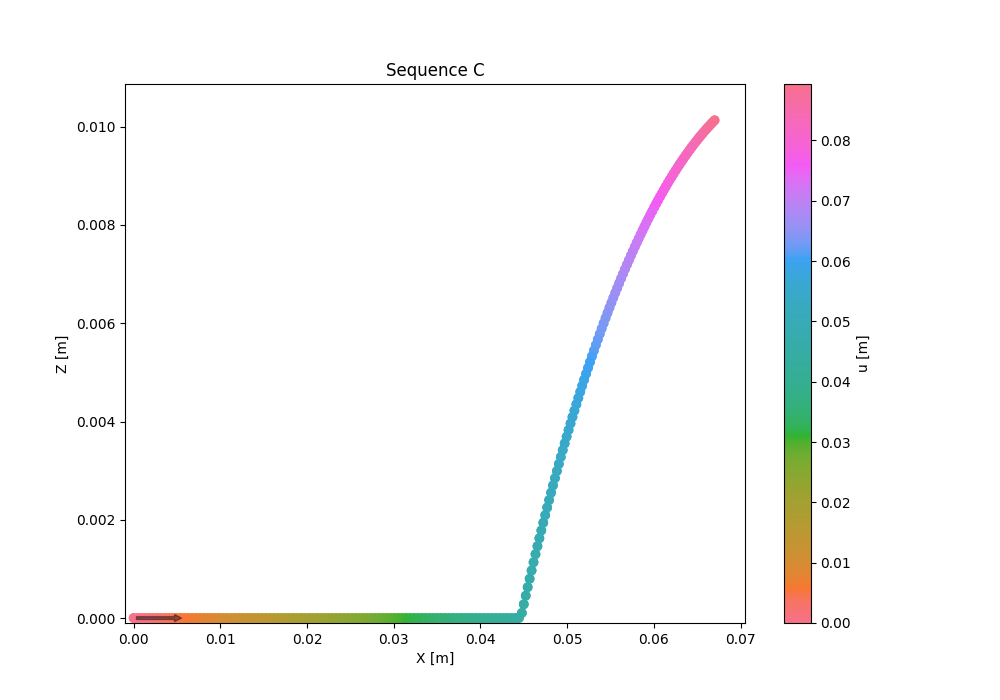
\includegraphics[width=\textwidth]{images/C.png}
            \end{subfigure}
            \caption{Sequence C is a symmetrical sequence where the forward and backward motion are following the same path. In this sequence we have first the middle block moving during the forward motion where the top block is moving first during the backward motion. Sequence D (Figure \ref{fig:appendix_seq_D}) is very similar except it is reversed.}
        \end{figure}
        
        \begin{figure}[h]
            \centering
            \begin{subfigure}{.2\textwidth}
            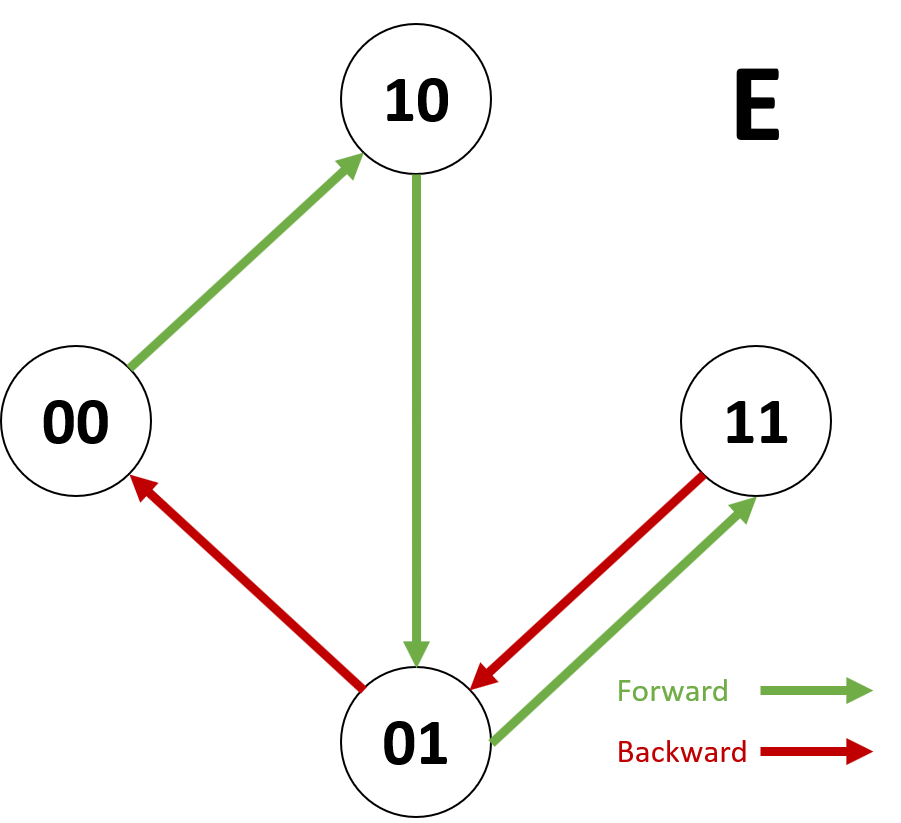
\includegraphics[width=\textwidth]{images/S_E.png}
            \end{subfigure}%
            \begin{subfigure}{.6\textwidth}
            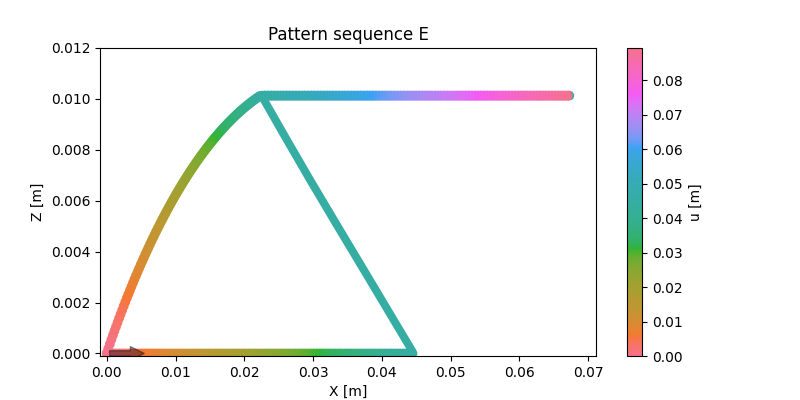
\includegraphics[width=\textwidth]{images/E.png}
            \end{subfigure}
            \caption{Sequence E is our first sequence with a avalanche mechanism where two blocks swap positions. This happens in the middle of the forward motion. We can see here that after moving horizontally, the legs is \textit{snapping} to go to another position without having motion for the actuator, producing this triangle shape. Sequence F (Figure \ref{fig:appendix_seq_F} is performing similarly but \textit{reversed}.}
        \end{figure}
        
        \begin{figure}[h]
            \centering
            \begin{subfigure}{.2\textwidth}
            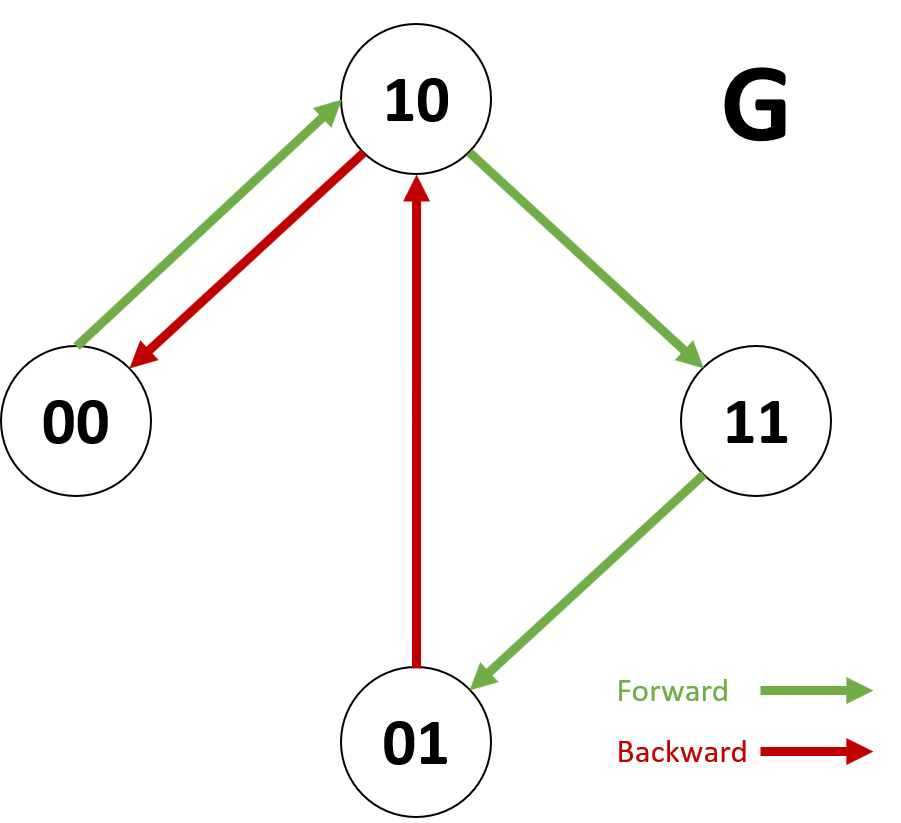
\includegraphics[width=\textwidth]{images/S_G.png}
            \end{subfigure}%
            \begin{subfigure}{.6\textwidth}
            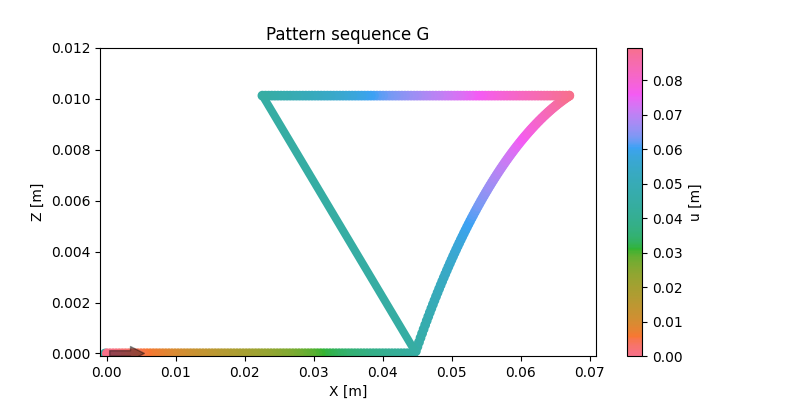
\includegraphics[width=\textwidth]{images/G.png}
            \end{subfigure}
            \caption{Sequence G is similar to sequence E and sequence F as there is also an avalanche effect that swap two blocks positions. But this time this swap motion happens during backward actuation instead of forward actuation. Sequence H (Figure \ref{fig:appendix_seq_H} is performing similarly but \textit{reversed}.}
        \end{figure}

        \begin{figure}[h]
            \centering
            \begin{subfigure}{.2\textwidth}
            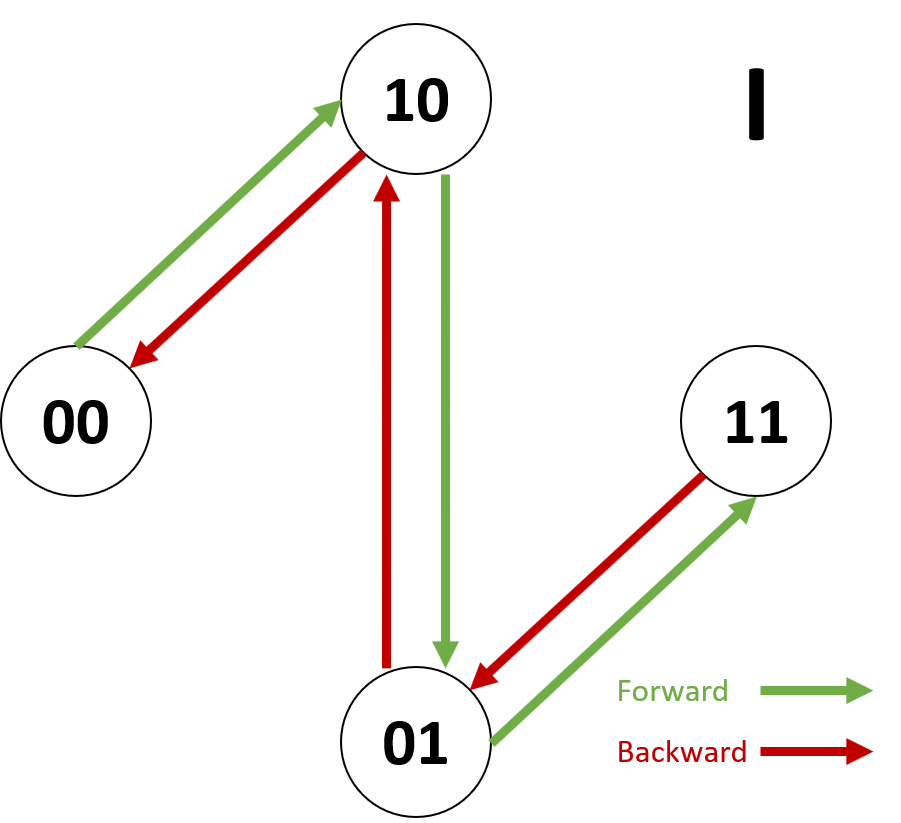
\includegraphics[width=\textwidth]{images/S_I.png}
            \end{subfigure}%
            \begin{subfigure}{.6\textwidth}
            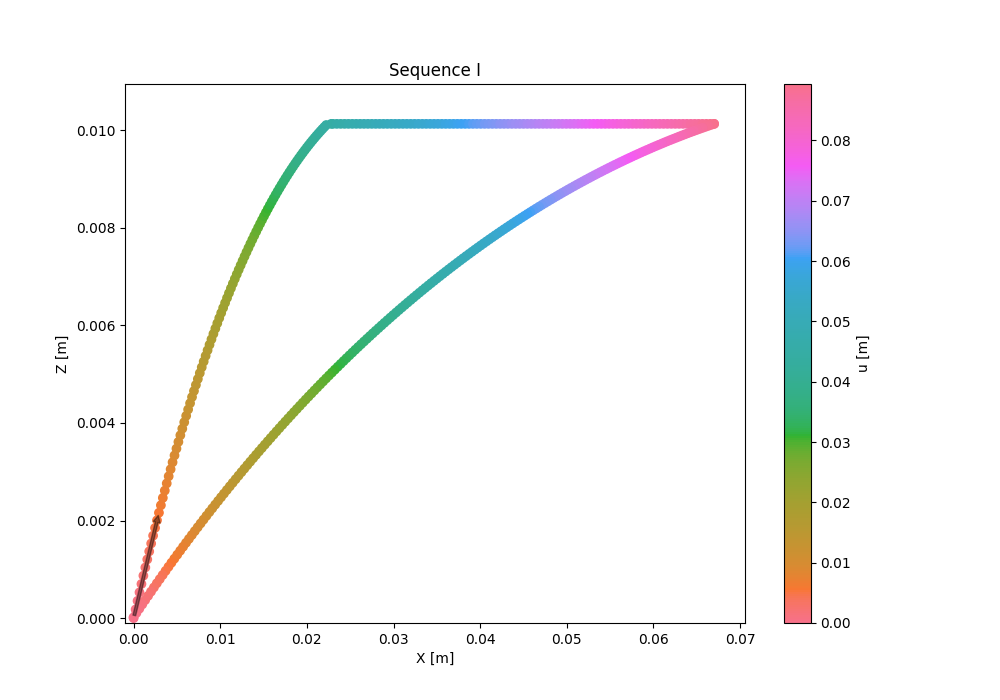
\includegraphics[width=\textwidth]{images/I.png}
            \end{subfigure}
            \caption{Sequence I is our only sequence with two avalanches mechanisms. This time we can see that the two blocks swap positions during forward and backward motions.}
        \end{figure}        
        
    \section{Drawings}
        Let's show what information are shown in the video of the simulation. We have an example of the kind of video you can expect as a result in Figure \ref{fig:drawing}. The simulation represent the robot in a schematic way, with a main frame represented by yellow blocks. On each corner we have a multistable joint as for the real robot. Actuators are not directly represented but we can identify two type of top blocks, green ones and magenta ones. Top blocks with the same color are linked together to the same actuator. Linking the blocks together we have springs and arms, respectively in gray and red. 
        
        \begin{figure}[h]
            \centering
            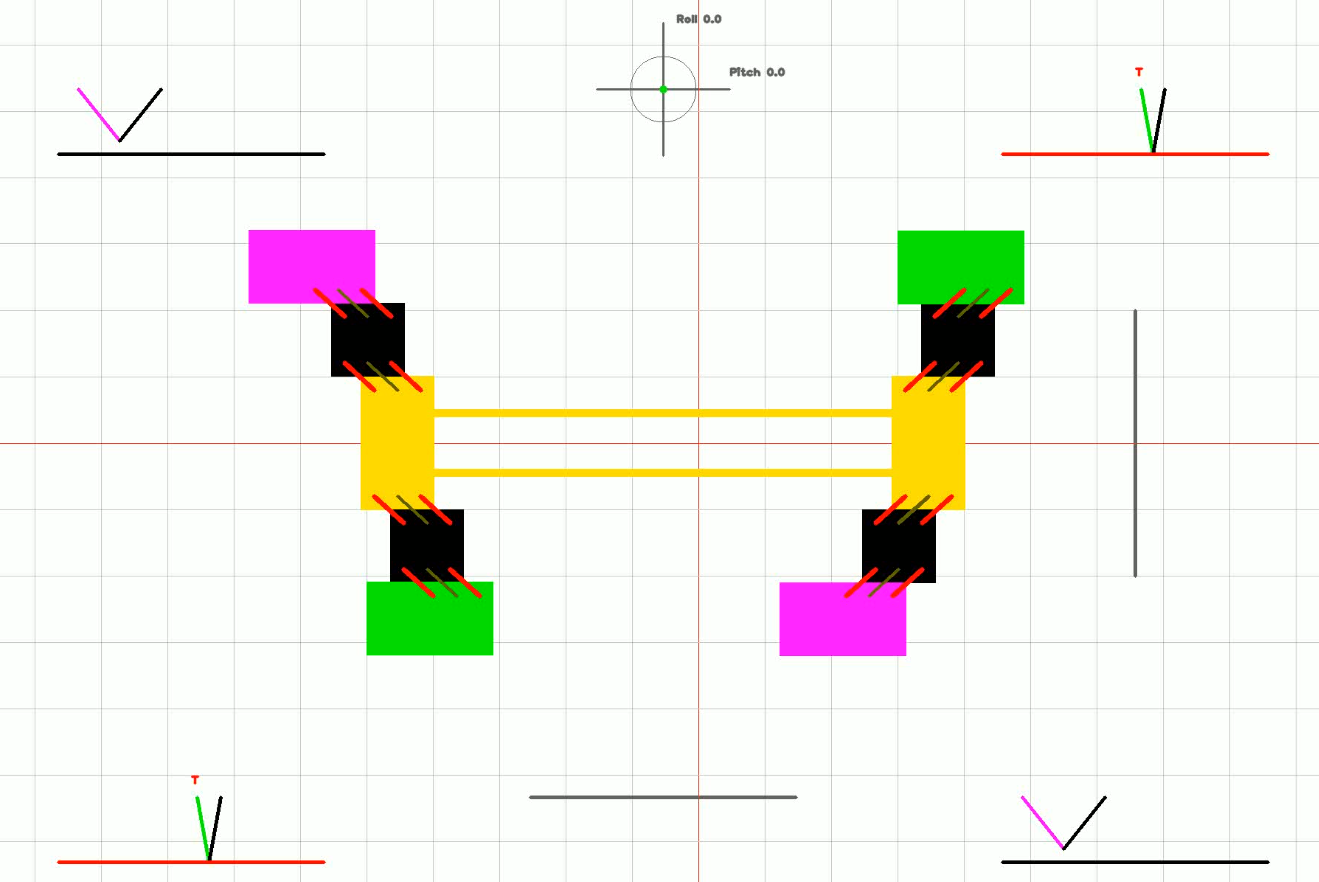
\includegraphics[width=0.8\textwidth]{images/drawing.png}
            \caption{Caption}
            \label{fig:drawing}
        \end{figure}
        
        The view of the robot is a top view as it allows us to understand how the sequences are happening. We have four smaller views on the four corner of the image. Those view represent a side view of each multistable joint. If we take the the example of the bottom left leg, we have a horizontal line which is a virtual representation of the ground position relative to the leg. We also have a green and black lines, the green line represent the arm that link the green block to the leg endpoint. The block line represent the arm that link the black block to the leg endpoint. The letter T and the red line are present when the leg is in contact with the ground. We can see in our case that two (green) legs are touching the ground while two others (magenta) are not.
        
    \section{Robot position}
        
        